%%%%%%%%%%%%%%%%%%%%%%%%%%%%%%%%%%%%%%%%%%%%%%%%%%%%%%%%%%%%%%%%%%%%%%
% LaTeX Template: Two Column Colour Article
%
% Source: http://www.howtotex.com/
% Feel free to distribute this template, but please keep the
% referal to howtotex.com.
% Date: Feb 2011
% 
%%%%%%%%%%%%%%%%%%%%%%%%%%%%%%%%%%%%%%%%%%%%%%%%%%%%%%%%%%%%%%%%%%%%%%
% How to use overleaf.com: 
%
% You edit the source code here on the left, and the preview on the
% right shows you the result within a few seconds.
%
% You can upload figures, bibliographies, custom classes and
% styles using the files menu.
%
% If you're new to LaTeX, the wikibook is a great place to start:
% http://en.wikibooks.org/wiki/LaTeX
%
%%%%%%%%%%%%%%%%%%%%%%%%%%%%%%%%%%%%%%%%%%%%%%%%%%%%%%%%%%%%%%%%%%%%%%
% adaptions made by wolfgang stoettner mail@stoettner.net
%%%%%%%%%%%%%%%%%%%%%%%%%%%%%%%%%%%%%%%%%%%%%%%%%%%%%%%%%%%%%%%%%%%%%%

%%% Preamble
\documentclass[	DIV=calc,%
							paper=a4,%
							fontsize=11pt,%
							twocolumn]{scrartcl} % KOMA-article class
\usepackage[french]{babel}	% English language/hyphenation
\usepackage[protrusion=true,expansion=true]{microtype}	% Better typography
\usepackage{amsmath,amsfonts,amsthm} % Math packages
\usepackage{pythontex} % Math packages
\usepackage[pdftex]{graphicx} % Enable pdflatex
\usepackage{wrapfig} % enable figure wrapping
\usepackage[svgnames]{xcolor} % Enabling colors by their 'svgnames'
\usepackage[hang, small,labelfont=bf,up,textfont=it,up]{caption} % Custom captions under/above floats
\usepackage{epstopdf} % Converts .eps to .pdf
\usepackage{subfig}	% Subfigures
\usepackage{booktabs} % Nicer tables
\usepackage{fix-cm}	% Custom fontsizes
\usepackage{booktabs} % prof. looking tables (www.en.wikibooks.org/wiki/LaTeX/Tables#Professional_tables)
\usepackage{float}
\usepackage{tgtermes}
\usepackage[T1]{fontenc}
\usepackage[utf8]{inputenc}
\usepackage{stackengine}
\usepackage{tikz,pgfplots}
\usepackage[export]{adjustbox}


%%% Custom sectioning (sectsty package)
\usepackage{sectsty} % Custom sectioning (see below)
\allsectionsfont{%		% Change font of al section commands
	\usefont{OT1}{phv}{b}{n}%	% bch-b-n: CharterBT-Bold font
	}

\sectionfont{%		% Change font of \section command
	\usefont{OT1}{phv}{b}{n}%	% bch-b-n: CharterBT-Bold font
	}
%%% Headers and footers
\usepackage{fancyhdr} % Needed to define custom headers/footers
	\pagestyle{fancy} % Enabling the custom headers/footers
\usepackage{lastpage}	

% Header (empty)
\lhead{}
\chead{}
\rhead{\today}
% Footer (you may change this to your own needs)
\lfoot{\footnotesize \texttt{formulaire capteur} \textbullet \vspace{5pt} Antonin Kenzi}
\cfoot{}
\rfoot{\footnotesize page \thepage\ of \pageref{LastPage}}	% "Page 1 of 2"
\renewcommand{\headrulewidth}{0.0pt}
\renewcommand{\footrulewidth}{0.4pt}
\newcommand{\hformbar}[1]{\bigskip\hrule\vspace{5pt}} % creates a horizontal bar to separate formulae better; space adaptions can be made centrally here

\newcommand{\vformbar}[1]{\bigskip\vrule\vspace{5pt}} % creates a horizontal bar to separate formulae better; space adaptions can be made centrally here

%%% Creating an initial of the very first character of the content
\usepackage{lettrine}
\newcommand{\initial}[1]{%
     \lettrine[lines=3,lhang=0.3,nindent=0em]{
     				\color{DarkGoldenrod}
     				{\textsf{#1}}}{}}

%%% Title, author and date metadata
\usepackage{titling} % For custom titles

\newcommand{\HorRule}{\color{DarkGoldenrod}%	% Creating a horizontal rule
									  	\rule{\linewidth}{1pt}%
										}
\pretitle{\vspace{-30pt} \begin{flushleft} \HorRule 
				\fontsize{15}{15} \usefont{OT1}{phv}{b}{n} \color{DarkRed} \selectfont 
				}
\title{Formulaire Capteur} % Title of your article goes here
\posttitle{\par\end{flushleft}}
\preauthor{\vspace{-20pt} \begin{flushleft}\large \usefont{OT1}{phv}{b}{sl} \color{DarkRed}}
\author{Kenzi Antonin}	% Author name goes here
\postauthor{\vspace{-20pt} \footnotesize \usefont{OT1}{phv}{m}{sl} \color{Black}  \par\end{flushleft}\HorRule}
\date{\vspace{-30pt} \today} % No date
\newcounter{mycounter}
%%% wws: create a non-indented formula name
\newcommand{\formdesc}[1]{\noindent\textbf{#1} \addtocounter{mycounter}{1} \hfill \themycounter}

%%% Begin document -----------------------------------------------------------------
\begin{document}
\maketitle
\thispagestyle{fancy} 	% Enabling the custom headers/footers for the first page 
% The first character should be within \initial{}

\formdesc{Classification des mesurandes}

\footnotesize il existe plusieurs catégories de mesurandes : 
\begin{enumerate}
 \item Mécanique : déplacement, vitesse... 
 \item Électrique : courant, tension, charge
 \item Thermique : température flux thermique
 \item Magnétique : champ magnétique, perméabilité
 \item Radiation : lumière visible, rayon X, radiation
 \item Bio/chimique :  humidité, gaz, sucre, hormones 
\end{enumerate}

\hformbar

\formdesc{Capteur et chaînes d'acquisition}
\begin{figure}[H]
    \begin{center}
        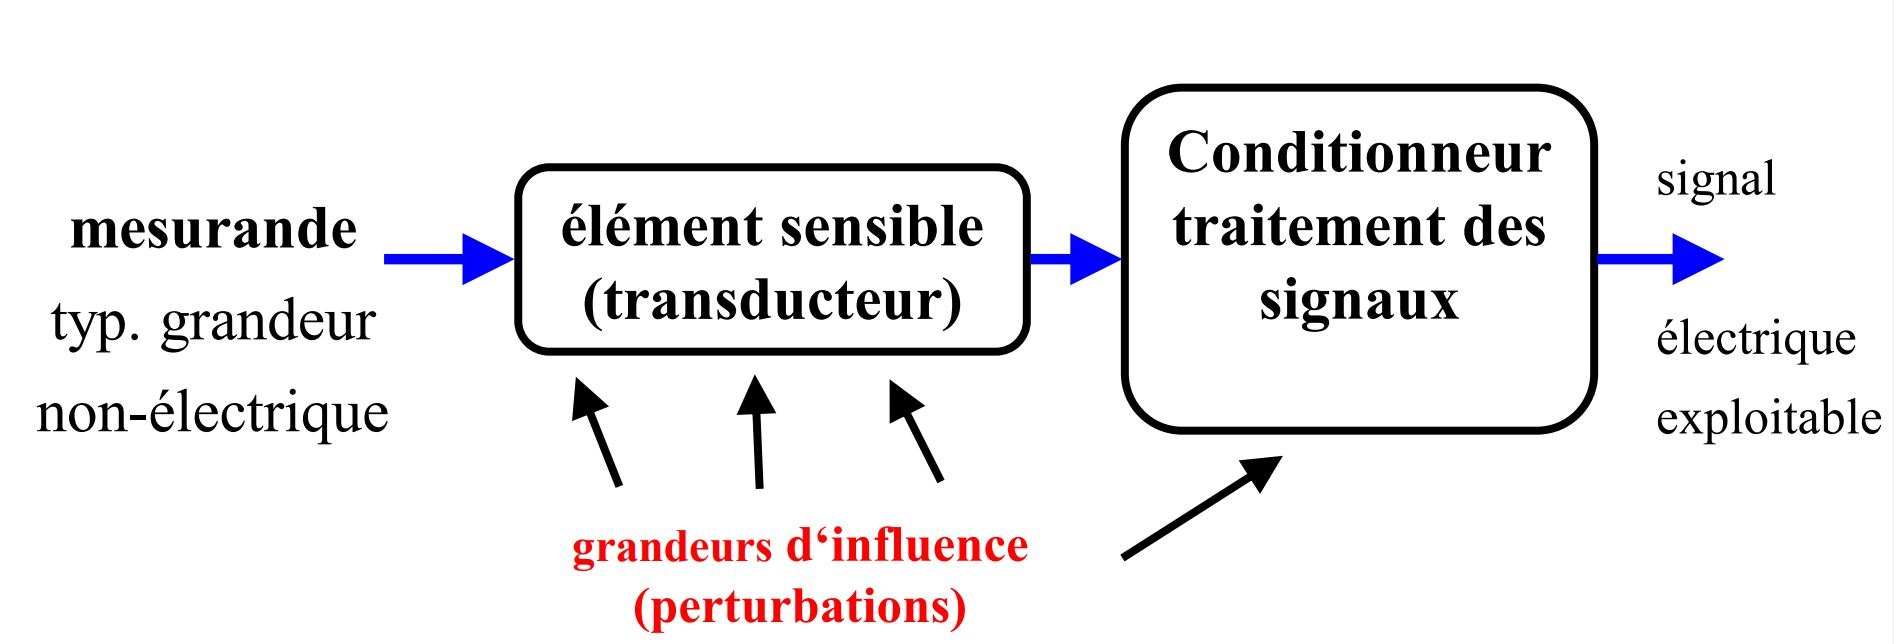
\includegraphics[width=0.3\textwidth]{img/capteur_influence.JPG}
        \caption{Illustration des influences}
        \label{fig:Illustration des influence}
    \end{center}
\end{figure}
Problèmes :
\begin{itemize}
 \item modifié par des grandeurs d'influence
 \item retard sur le signal
 \item un organe de mesure modifie l'environnement
\end{itemize}

\hformbar

\formdesc{Sensibilité du capteur}

{\hfill $ S = \cfrac{\Delta s}{\Delta m} \big |_mi$ \hfill }
\begin{figure}[H]
    \begin{center}
        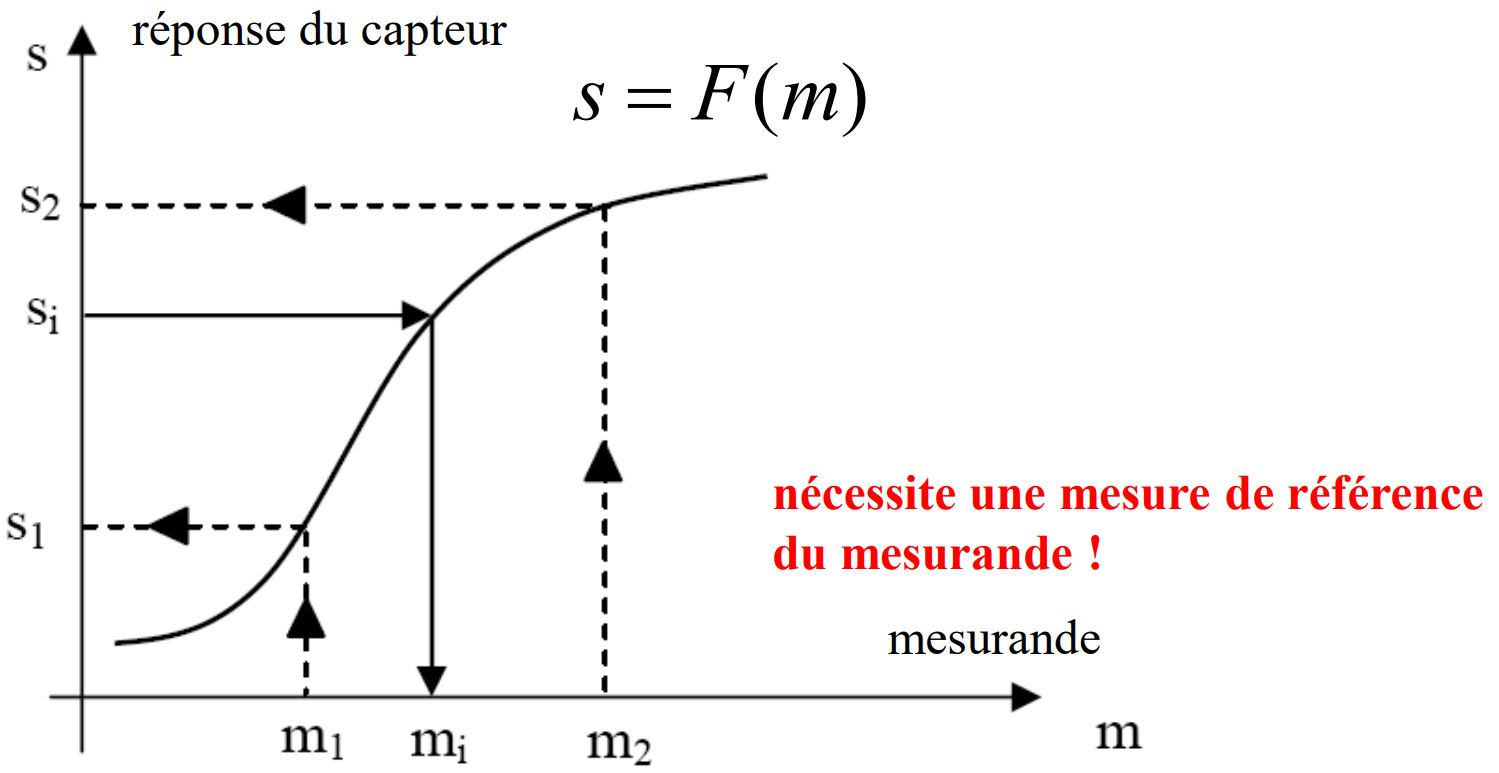
\includegraphics[width=0.3\textwidth]{img/Etalonage_statique.JPG}
        \caption{Etalonage Statique, Cas idéale}
        \label{fig:Etalonage Statique, Cas idéale}
    \end{center}
\end{figure}
\hformbar

\formdesc{Erreur de linéarité}
\begin{figure}[H]
    \begin{center}
        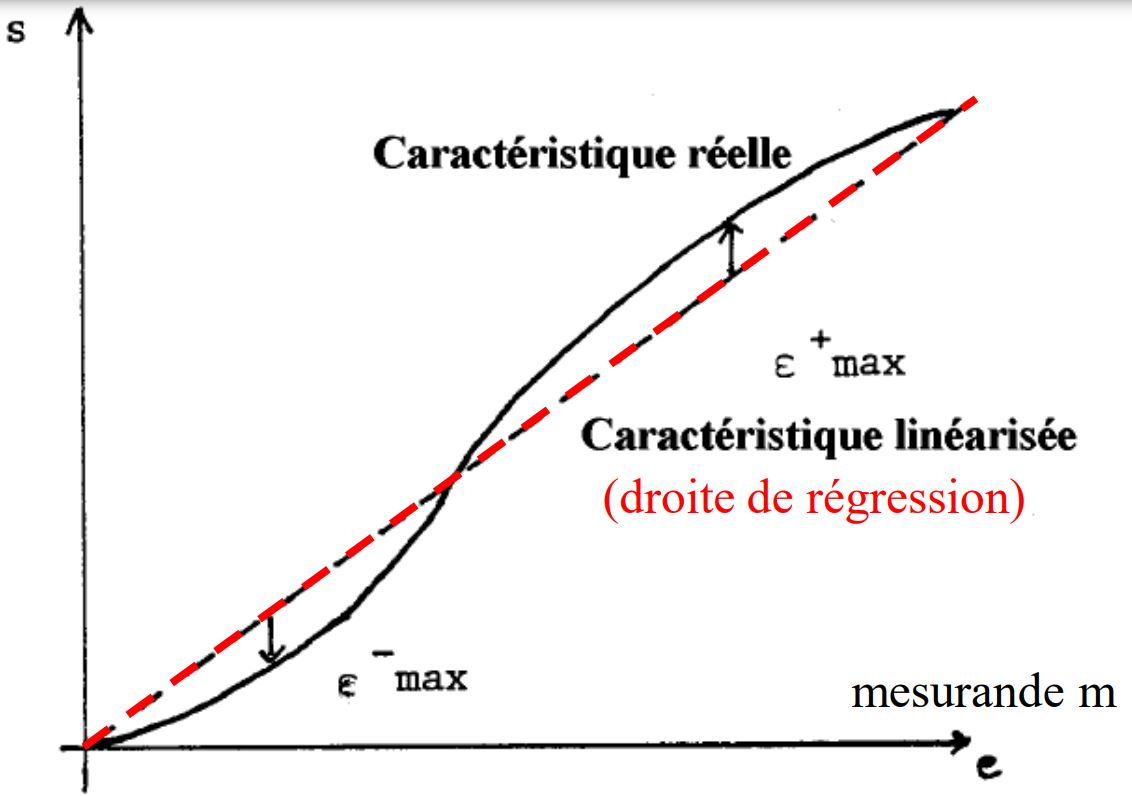
\includegraphics[width=0.2\textwidth]{img/linearite.JPG}
        \caption{Erreur de linéarité}
        \label{fig:Erreur de linéarité}
    \end{center}
\end{figure}
Elle s'exprime en \%, soit l'erreur relative maximale entre la droite de régression et la caractéristique réelle.

\formdesc{Résolution}

Définition : La résolution est la plus petite variation du mesurande que le capteur est capable de definir.
Son étendue de mesure est découpé en 3 zones : 
\begin{itemize}
    \item Nominale : plage nominale de mesurande (fonctionnement normal)
    \item Non-destruction : hors spécification, mais dans l'"absolute maximum rating"
    \item Destructive : altération permanente des caractéristiques de mesure.
\end{itemize}

\hformbar

\formdesc{Rapidité d'un capteur}

\begin{itemize}
    \item Bande passante, plage de fréquence ou le gain est supérieur à 3dB du plateau
    \item Temps de réponse, temps nécessaire pour que le capteur atteigne 95 \% de la valeur finale.
\end{itemize}
Les deux paramètres sont intrinsèquement liés. 

{\hfill $T_{rep} = 3 \cdot \tau = \cfrac{3}{2\pi \cdot f_c}$ \hfill}

\hformbar

\formdesc{Erreur de mesure}

Deux genres d'erreur:
\begin{itemize}
    \item Systématique : Dérive, mauvaise utilisation, vieillissement.
    \item Accidentelles (aléatoire) : Bruit, parasite, environnement.
\end{itemize}
En étudiant la densité de probabilité, on peut ressortir deux comportements : 
\begin{itemize}
    \item Justesse, Moyenne de mesurande proche de la valeur réelle
    \item Fidélité (répétabilité), Erreur accidentelle faible (variance faible)
\end{itemize}
lorsque les deux paramètres sont bons, on parle de précision

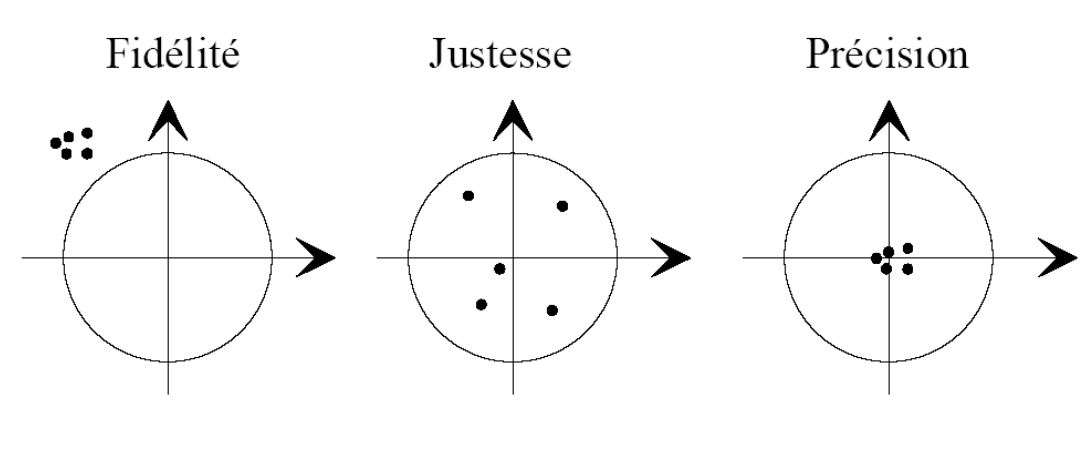
\includegraphics[width=0.49\textwidth,center]{img/justesse.JPG}

\hformbar


\formdesc{Choix du capteur}
\begin{itemize}
    \item principe physique 
    \item performance(résolution, précision, plage de mesure)
    \item Grandeur d'influence 
    \item encombrement
    \item prix
    \item fiabilité, MTBF : Mean Time Between Failures
\end{itemize}

$MTBF = \cfrac{1}{\lambda}$

$\lambda : taux de defaillance = \cfrac{1}{N_{pop}}\cfrac{\Delta N_{def}}{\Delta t} $
\newpage

\formdesc{Capteur résistif}

Thermistance :
les thermistances de platine sont conçues avec deux méthodes : 
\begin{itemize}
    \item fil de platine enroulé, précis, mais chère (1000.-)
    \item film mince de platine (env.$1\mu m$), réponse rapide et abordable (10.-)
\end{itemize}
Lorsque l'on parle de PT-X,  on parle de la sonde de platine dont la valeur à 0°C est de X $\Omega$
le coefficient $\alpha$ typique est de 0.385 \%/°C et une précision de 0.1 à 1\%

la résistance s'exprime par :

{\hfill $R_{T} = R_0 (1+\alpha T)$ \hfill}

\begin{figure}[H]
    \begin{center}
        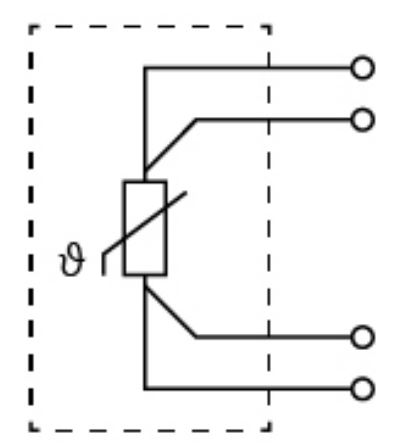
\includegraphics[width=0.15\textwidth]{img/PT.JPG}
        \caption{Symbole IEC normalisé de la PT}
        \label{fig:symbole_PT}
    \end{center}
\end{figure}


\hformbar

\formdesc{Conditionneurs pour capteur résistif}

conditionneur linéaire à source de courant :

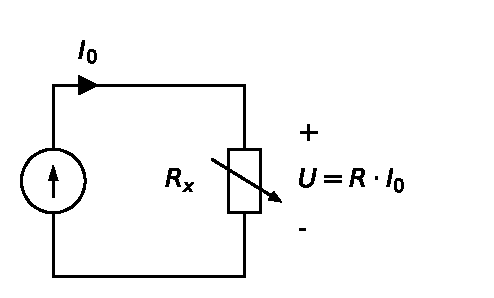
\includegraphics[width = 0.3\textwidth,center]{img/condi_cur.pdf}

conditionneur non-linéaire type "diviseur de tension" :

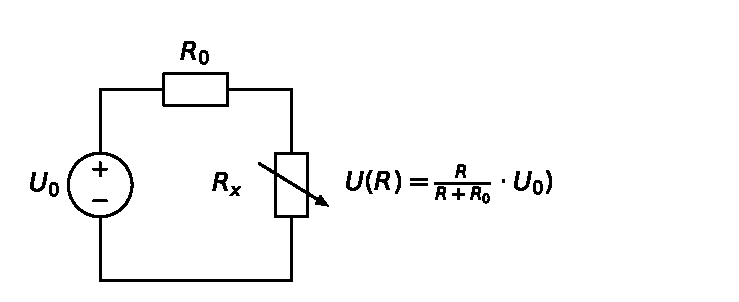
\includegraphics[width = 0.5\textwidth,center]{img/condi_ten.pdf}

$S_{cond} = \cfrac{\Delta U }{\Delta R } = \cfrac{d U }{d R } = \cfrac{R_0 }{(R_0 + R_{nom})^2}\cdot U_0$
$R_{0,opti} = R_{nom}$
$U(R)$ varie jusqu'à $U_0/2$

Pont de Wheatstone, tension de déséquilibre:

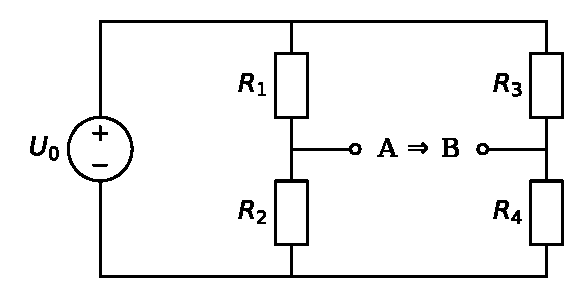
\includegraphics[width = 0.3\textwidth,center]{img/wheastone.pdf}

$u_m = u_a-u_b = \cfrac{R2}{R1+R2}-\cfrac{R4}{R3+R4} \cdot U_0$

$u_m = 0 \leftrightarrow R1R4=R2R3$

en mode "nulling"

R2 = capteur

R4 programée $R_{2,capt} = R_{4,prog} = \cfrac{R1}{R3}$

Avantages :

\begin{itemize}
    \item indépendant de la tension d'alimentation U0
    \item indépendant de la précision de mesure de Um, il faut juste pouvoir détecter précisément "zéro".
    \item indépendant d'un courant de mesure de Um
\end{itemize}

Inconvénients :

- faible bande passante, que possible pour des mesurandes statiques

$R2 = R_0 + \Delta R_c$

$R1 = R3 = R4 = R0$

$u_m = \bigg(\cfrac{R_0 + \Delta R_c}{2 R_0 + \Delta R_c}-\cfrac{1}{2}\bigg) U_0 = \bigg(\cfrac{\Delta R_c}{4 R_0 + 2\Delta R_c}\bigg) U_0$

$S_{cond} = \cfrac{U_0}{4R}$


montage différentiel: "push-pull

$R1 = R_0 + \Delta R_c$

$R2 = R_0 - \Delta R_c$

$R3 = R4 = R0$

$u_m(\Delta R_c) = \cfrac{U_0}{2R_0}\cdot \Delta R_c $

$S_{cond} = \cfrac{U_0}{2R_0}$

utilisation du pont de Wheatstone en mode 4/4 différentiel

$R1 = R4 = R_0 - \Delta R_c$

$R2 = R3 = R_0 + \Delta R_c$

$u_m(\Delta R_c) = \cfrac{U_0}{R_0}\cdot \Delta R_c $

$S_{cond} = \cfrac{U_0}{R_0}$


\hformbar

\formdesc{Amplificateur différentiel}

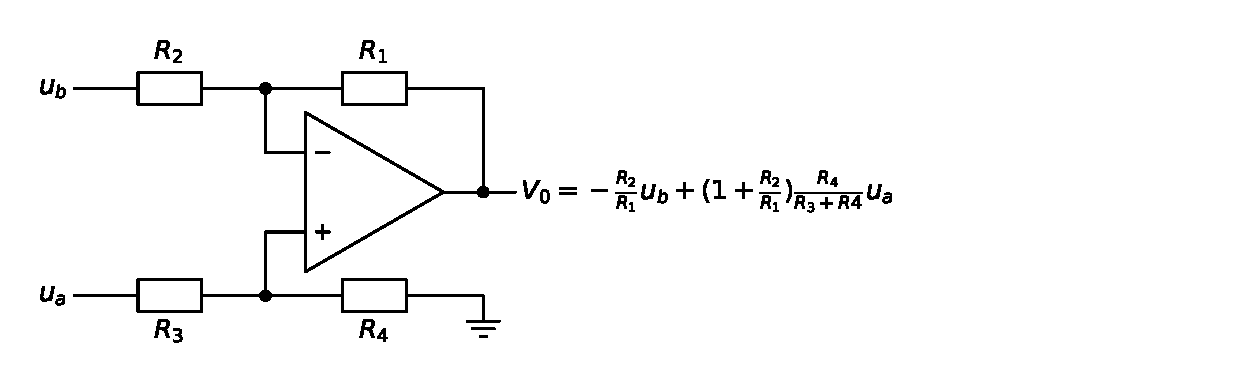
\includegraphics[width = 0.55\textwidth,center,trim={0 0 5cm 0},clip]{img/Ampli.pdf}

$u_d = u_a - u_b$

$u_c = \cfrac{u_a + u_b}{2}$

$V_0 = G_c \cdot u_c + G_d \cdot u_d $

$Gc = \cfrac{V_o}{E_c}\bigg|_{Ed = 0} = \cfrac{R4R1-R2R3}{R1(R3+R4)}$


$Gd = \cfrac{V_o}{E_d}\bigg|_{Ec = 0} = \cfrac{1}{2}\bigg[\cfrac{R2}{R1}+\bigg(1+ \cfrac{R2}{R1}\bigg)\cfrac{R4}{R3+R4}\bigg]$

$CMRR = \cfrac{G_d}{G_c}$



\hformbar

\formdesc{électromagnétisme}

Phénomènes physiques exploités
\begin{itemize}
    \item variation de la réluctance d‘un circuit magnétique (p.ex. variation de l‘entrefer)
    \item variation du facteur de couplage entre 2 ou plusieurs bobines
    \item détection des pertes ohmiques crées par des courants de Foucault induits dans une cible conductrice
    \item variation de l‘inductance due au champ opposé crée par les courants de Foucault
    \item loi d‘induction de Faraday (tension induite par un champ variable)
\end{itemize}

Rappel : 

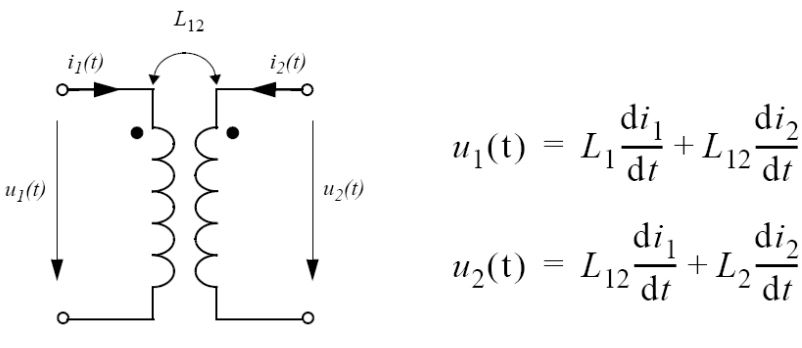
\includegraphics[width = 0.4\textwidth,center]{img/Rappel_ind.JPG}

Facteur de couplage : $ k = \sqrt{\cfrac{L_{12}^2}{L_1 L_2}}$

Capteur de proximité : effets physiques (1/2)
\begin{itemize}
    \item bobine seule, sans présence de cible
    \begin{itemize}
        \item effet de peau : fréquence élevée $\Rightarrow$ résistance augmente
        \item auto-résonance avec la capacité parasitaire
    \end{itemize}
    \item cible conducteur non ferromagnétique
    \begin{itemize}
        \item Courants de Foucault induits $\Rightarrow$ résistance équivalente augmente
        \item champ magnétique induit opposé $\Rightarrow$ inductance équivalente diminue
    \end{itemize}
    \item cible conducteur ferromagnétique non-conducteur (~ferrite)
    \begin{itemize}
        \item effet de reluctance, concentration du champ magnétique $\Rightarrow$ inductance augmente 
    \end{itemize}
    \item cible conducteur ferromagnétique conducteur (p.ex. fer)
    \begin{itemize}
        \item à basse fréquence : peu de courants de Foucault, augmentation de l'inductance
        \item à haute fréquence : courants de Foucault élevés, diminution de l'inductance
    \end{itemize}
\end{itemize}


Capteurs inductifs et à courant de Foucault et Circuit de résonance


\begin{enumerate}
    \item Bobine idéale ($R_b = 0$)
        \begin{itemize}
            \item Diagramme de Bode de $H(j\omega)$
            \item Affichage de H(L) dans le plan complexe
            \item Fonction de Möbius
        \end{itemize}
    \item Bobine nonidéale ($R_b \neq 0$)
        \begin{itemize}
            \item Fréquence de résonnance
            \item Choix optimal de R0
        \end{itemize}
\end{enumerate}

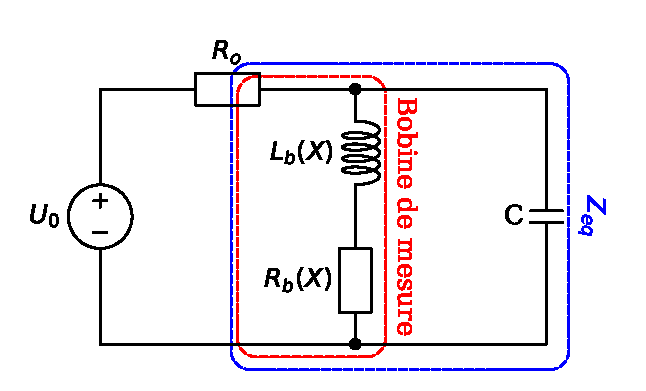
\includegraphics[width = 0.4\textwidth,center]{img/circuit_res.pdf}

Bobine Idéale :

$Z_{para} = \cfrac{j\omega L_b}{1+(j\omega)^2L_bC}$

$\underline{H}(j\omega,Lb) = \cfrac{Z_{para} }{Z_{para} + R_0} = \cfrac{j\omega L_b}{R0 + j\omega L_b+(j\omega)^2R_0L_bC}$

Sous forme de Bode : 


$\underline{H}(j\omega,Lb) = \cfrac{j\omega L_b/R0}{1+ \underbrace{\cfrac{L_b}{R_0}}_{\cfrac{2\zeta}{\omega_r}}j\omega + \underbrace{\cfrac{1}{1/(L_bC)}}_{\cfrac{1}{\omega_r^2}}(j\omega)^2}$

$\omega_r = \cfrac{1}{\sqrt{L_b C}}$ \quad $\zeta = \cfrac{L_b}{2R_0\sqrt{L_b C}}$


Bobine réelle :

$\omega_res = \sqrt{\cfrac{1}{L_b C} - \cfrac{R_b^2}{L_b^2}}$ \quad $Z_{para,res} = \cfrac{L_b}{R_b C} = R_{para,res}$

$S_{cond} = \biggl|\cfrac{dH}{dZ_{bobine}}\biggr|$
\end{document}